% 以下は編集作業時に各人のフォーマットがズレるので変更しないこと。
\documentclass[
  paper={202mm,277mm},
  twoside,
  twocolumn,
  head_space=24mm,
  foot_space=28mm,
  gutter=32mm,
  line_length=71mm,
  column_gap=6mm,
  jafontsize=9pt,
]{jlreq}
\usepackage{laboticgate}

% ページ番号を設定。編集時に調整するため変更不要。
\setcounter{page}{1}

% 記事番号を設定。編集時に調整するため変更不要。
\setchapter{1}

% レイアウトの都合上、フォントサイズの若干の調整はOK。
\title{26pt}{らぼちっく;げーと\\ \LaTeX テンプレート v1.4}
\titleskip{-7mm}

% 各ページ下部のノンブル横に印刷されるタイトル。改行を入れないこと。
\footertitle{らぼちっく;げーと \LaTeX テンプレート v1.4}

% 記事タイトル下部に印刷される記事の概要。
\summary{らぼちっく;げーとの同人誌で使う記事テンプレートです。}
\summaryskip{-10mm}

% 日付は空のままにしておくこと。
\date{}

% 著者名(ハンドルネーム可)
\author{ぺんぎんさん}

% 所属(表示しない場合はコメントアウトしておく)
%\affiliation{らぼちっく;げーと}

% SNSアカウント(表示しない場合はコメントアウトしておく)
\social{X/Twitter}{@penguin2716}

% メールアドレス(表示しない場合はコメントアウトしておく)
%\email{laboticgate@example.com}

% 変更しないこと
\begin{document}
\maketitle
\thispagestyle{fancy}
\section{このテンプレートについて}
この \LaTeX テンプレートは、技術系同人サークル「らぼちっく;げーと」が同人誌を制作する際に、各記事の執筆者の皆様に利用してもらっているものです。本テンプレートをコピーして、各自の記事を作成してください。

\section{節、項、目による文章構成}
らぼちく本では、記事の単位をChapterとし、各記事の中では \verb=\section{節タイトル}= 、 \verb=\subsection{項タイトル}= 、 \verb=\subsubsection{目タイトル}= の3段階のレベルで分けられるようになっています。節、項、目にはそれぞれ番号は振られません。\verb=\section{節タイトル}= とすると、このようになります。

\subsection{項タイトル}
\verb=\subsection{項タイトル}= とすると、このようになります。

\subsubsection{目タイトル}
\verb=\subsubsection{目タイトル}= とすると、このようになります。

\section{記事の書き方}
\subsection{タイトル、概要、プロフィール}
\verb=main.tex=に記載してください。

\subsection{本文}
\verb=content.tex=に記事内容を作成してください。

\subsection{等幅フォント}
コマンド名やファイル名などで等幅フォントを使用したい場合は \verb|\verb=monospace=| のように入力してください。 \verb=monospace= のように表示されます(HTMLの\verb|<pre>|タグに相当するものです)。左右の記号は \verb|=| 以外でも構いません。特殊文字を含まない場合は \verb|\texttt{monospace}| としてもよいです(\texttt{monospace} のように表示されます)。

\subsection{URL}
URLは \verb=\url{http://www.example.com}= のように入力すると \url{http://www.example.com} のように表示されます。

\subsection{数式}
数式は \LaTeX 標準のものが利用できます。

\subsection{ルビを\ruby{振}{ふ}る}
ルビは \verb=\ruby{探偵}{プライベート・アイ}= のように入力すると \ruby{探偵}{プライベート・アイ} のように表示されます。

\subsection{引用符(``'', `')}
引用符は\verb=``文字列''=のように記載してください。``文字列''のように表示されます。ダブルクォートではなくシングルクォートを利用する場合、\verb=`文字列'=のようにすると、`文字列'のように表示されます。なお\verb=`=はバッククォートで、日本語配列のキーボードならShift+@、英語配列なら1キーの左にあるキーをタイプして入力してください(英語配列のHHKBの場合は最上段の最右のキーです)。

\subsection{列挙(箇条書き)}
番号を振らずに箇条書きとしたい場合、\verb=itemize=を使います。

\begin{itemize}
    \item 1つ目
    \item 2つ目
\end{itemize}

\verb=\item[★]=のようにして中点を別の文字に置き換えることもできます。

\begin{itemize}
    \item[★ ] 1つ目
    \item[♫ ] 2つ目
\end{itemize}

番号を振りたい場合、\verb=enumerate=を使います。

\begin{enumerate}
    \item 1つ目
    \item 2つ目
\end{enumerate}

\subsection{余白と改ページ}
レイアウトの都合で、本文や図表を上下左右に少しだけ動かしたい場合、\verb=\vspace{1mm}=で1mm上に、\verb=\hspace{1mm}=で1mm右に移動できます。多用すると \LaTeX の自動組版と整合性が取りにくくなるケースがあるため、「どうしても」という場合以外は利用しないことをおすすめします。

節、項、目、段落等をページ上部から始めたい場合、\verb=\newpage=を使うことでページを改めることができます。基本的には \LaTeX の自動組版に任せるのがよいですが、レイアウトを調整したい場合には利用できます。

\section{図表の入れ方}
\subsection{図}
らぼちく本のC99表紙画像の一部を例とすると、画像は図\ref{portrait-image}のように掲載することも、図\ref{landscape-image}のように2段組をぶち抜きで掲載することもできます。違いは\verb=figure=が\verb=figure*=になっているだけで、それ以外の記載方法は同じです。

画像を掲載する際は、ImageMagick等でグレースケール化してください。また、印刷時に画像のピクセルが見えたりボケたりする可能性があるため、もし可能であれば600dpi程度以上の解像度を確保してください(通常サイズなら横幅1677px以上、ぶち抜きサイズなら横幅3496px以上が推奨されます)。また、図中に文字が記載されており、読者に読ませる必要がある場合、フォントサイズに配慮してください。小さなフォントサイズだと、印刷後に読めない可能性があります。

\begin{figure}[t]
  \begin{center}
    
\includegraphics[width=\linewidth]{images/c99-square.png}
  \end{center}
  \caption{通常の画像掲載例}
  \label{portrait-image}
\end{figure}

\begin{figure}[t]
  \begin{center}
    
\includegraphics[height=.70\linewidth,angle=-90]{images/c99-square.png}
  \end{center}
  \caption{右に90度回転、70\%に縮小した画像掲載例}
  \label{lenna-square-angled}
\end{figure}

\begin{figure*}[t]
  \begin{center}
    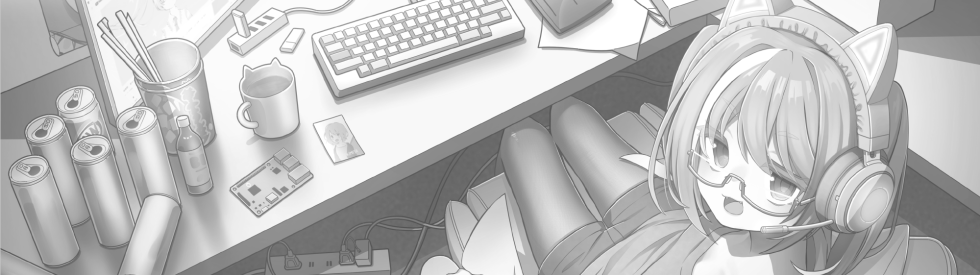
\includegraphics[width=\linewidth]{images/c99-header.png}
  \end{center}
  \caption{2段組ぶち抜きで図を掲載する例}
  \label{landscape-image}
\end{figure*}

\subsection{表}
表は表\ref{desktop-configurations}のように掲載するか、横長で文字が小さくなってしまう場合は表\ref{desktop-configurations-wide}のように2段組をぶち抜いて掲載します。フォントサイズは\verb=\scalebox{0.9}{...}=のように表全体のサイズを調整することで行います。

\begin{table}[t]
  \caption{通常の表掲載例}
  \label{desktop-configurations}
  \begin{center}
    \scalebox{0.7}{
      \begin{tabular}{ll}
        \toprule
        部品 & 型番 \\
        \midrule
        CPU & AMD Ryzen\texttrademark 5 5600G \\
        M/B & ASUS TUF GAMING X570-PLUS \\
        RAM & CORSAIR VENGEANCE\textregistered  LPX 32GB \\
        GPU & ZOTAC GAMING GeForce GTX 1660 SUPER Twin Fan \\
        PSU & ANTEC NeoECO GOLD NE750 \\
        Case & ANTEC P100 \\
        \bottomrule
      \end{tabular}
    }
    \end{center}
\end{table}

\begin{table*}[t]
  \caption{2段組ぶち抜きで表を掲載する例}
  \label{desktop-configurations-wide}
  \begin{center}
    \scalebox{1.0}{
      \begin{tabular}{ll}
        \toprule
        部品 & 型番 \\
        \midrule
        CPU & AMD Ryzen\texttrademark 5 5600G \\
        M/B & ASUS TUF GAMING X570-PLUS \\
        RAM & CORSAIR VENGEANCE\textregistered  LPX 32GB \\
        GPU & ZOTAC GAMING GeForce GTX 1660 SUPER Twin Fan \\
        PSU & ANTEC NeoECO GOLD NE750 \\
        Case & ANTEC P100 \\
        \bottomrule
      \end{tabular}
    }
    \end{center}
\end{table*}


\subsection{コードブロック}
コードブロックは次のように掲載します。フォントサイズが小さくて読めない場合は、\verb=lstlisting=の\verb=basicstyle=オプションを編集し調整することもできます。

\begin{lstlisting}
$ pciconf -lv
iwm0@pci0:2:0:0:	class=0x028000 rev=0x78 hdr=0x00 vendor=0x8086 device=0x24fd subvendor=0x8086 subdevice=0x0010
    vendor     = 'Intel Corporation'
    device     = 'Wireless 8265 / 8275'
    class      = network
\end{lstlisting}

また、リスト\ref{sample-codeblock}のように2段組をぶち抜きで掲載することもできます。その場合は\verb=figure*=で囲い、キャプションやラベルは\verb=lstlisting=のオプションとして記載してください。

\begin{figure*}[tb]
  \begin{lstlisting}[caption={2段組ぶち抜きでコードブロックを掲載する例},label={sample-codeblock},captionpos=b,basicstyle=\ttfamily\textsf\tiny\fontsize{6.3pt}{6.3pt}\selectfont]
$ lspci
00:00.0 Host bridge: Intel Corporation Device 4621 (rev 02)
00:02.0 VGA compatible controller: Intel Corporation Alder Lake-P GT2 [Iris Xe Graphics] (rev 0c)
00:04.0 Signal processing controller: Intel Corporation Alder Lake Innovation Platform Framework Processor Participant (rev 02)
00:05.0 Multimedia controller: Intel Corporation Alder Lake Imaging Signal Processor (rev 02)
00:06.0 PCI bridge: Intel Corporation 12th Gen Core Processor PCI Express x4 Controller #0 (rev 02)
00:07.0 PCI bridge: Intel Corporation Alder Lake-P Thunderbolt 4 PCI Express Root Port #0 (rev 02)
00:07.2 PCI bridge: Intel Corporation Alder Lake-P Thunderbolt 4 PCI Express Root Port #2 (rev 02)
00:08.0 System peripheral: Intel Corporation 12th Gen Core Processor Gaussian & Neural Accelerator (rev 02)
00:0a.0 Signal processing controller: Intel Corporation Platform Monitoring Technology (rev 01)
00:0d.0 USB controller: Intel Corporation Alder Lake-P Thunderbolt 4 USB Controller (rev 02)
00:0d.2 USB controller: Intel Corporation Alder Lake-P Thunderbolt 4 NHI #0 (rev 02)
00:0d.3 USB controller: Intel Corporation Alder Lake-P Thunderbolt 4 NHI #1 (rev 02)
00:14.0 USB controller: Intel Corporation Alder Lake PCH USB 3.2 xHCI Host Controller (rev 01)
00:14.2 RAM memory: Intel Corporation Alder Lake PCH Shared SRAM (rev 01)
00:14.3 Network controller: Intel Corporation Alder Lake-P PCH CNVi WiFi (rev 01)
00:15.0 Serial bus controller: Intel Corporation Alder Lake PCH Serial IO I2C Controller #0 (rev 01)
...
  \end{lstlisting}
\end{figure*}


\section{各種外部引用の方法}
\subsection{参考文献}
参考文献を掲載するには \verb=\cite{...}= のように...に指定の参考文献タグをつけて記載します。参考文献タグはに自身がcites.bibに\verb=@misc{...,= として登録することで設定できます。たとえば、\verb=\cite{iwm4}= と参考文献\cite{iwm4}をつけると、左記のとおり参考文献のリンクが生成されます。参考文献は記事の最後にまとめて列挙され、本文を読む邪魔にならない仕組みになっています。

\subsection{引用}
別の文献等から一部を引用する場合は、\verb=\begin{quotation}...\end{quotation}=を使って掲載します。引用元は参考文献を示してください。

\begin{quotation}
  吾輩は猫である。名前はまだない。
\end{quotation}

\subsection{脚注}
脚注はURLや簡易な注釈をつけたい場合に利用します。\verb=\footnote{...}= というように表記して、文章を補足することができます\footnote{\url{https://www.google.co.jp/search?q=footnote+tex}}。

\section{図と表の配置を調整する}
\subsection{配置調整のための命令}
\LaTeX では、次の図および表を挿入するための命令に対し、それをどこに配置するか(ページ上部、下部など)を指定できます。画像、表それぞれ、次のようにbegin命令の末尾に \verb=[t]= や \verb=[htb]= のような記載ができ、これによって記載位置を指定します。

\begin{itemize}
    \item 画像  \verb=\begin{figure}[t]= 
    \item 表 \verb=\begin{table}[htb]= 
\end{itemize}

とはいえ、このように配置を指定しても \LaTeX の組版システムによって調整されるため、必ずしも期待通りの位置に図表が配置されない場合もあります。

\subsection{基本的な配置の考え方}
配置の基本的な考えを数パターン、表\ref{htbp}で紹介します。htbpの順番に記述し、左から順番に配置場所が優先されます。下記ではよく使う配置のみを紹介します。

\begin{table}[htb]
  \caption{よく使う配置命令の一覧}
  \label{htbp}
  \begin{center}
    \scalebox{0.65}{
      \begin{tabular}{ll}
        \toprule
        \url{[...]} & 説明 \\
        \midrule
        \url{[t]} & 紙面の上部に配置する。図やぶち抜きでよく使う。 \\
        \url{[tb]} & 紙面の上部か下部に配置、表でよく使う。 \\
        \url{[htb]} & 本文中に記載した位置か、上部、下部どこかに載せる。\\
         & この表も \url{[htb]} で記述している。 \\
        \url{[b]} & 紙面の下部に配置する。表で使うが \\
        & 文章が足りない場合にうまくいかないことが多い。 \\
        \url{[h]} & ここ(書かれた場所)に配置する。\\
        & 文章が足りない場合にうまくいかないことが多い。 \\
        & このhは余白がうまく調整できていないこともある。 \\
        \bottomrule
      \end{tabular}
    }
    \end{center}
\end{table}

\subsection{考えるな、感じろ}
と、ここまで配置方法の解説を書いてきましたが、そもそもある程度の文章量がないと、思ったように図表が配置されません。
特に、1ページに複数図表がおかれる場合は、実際は細かい調整が必要なことも多く、それなりの経験と工夫が必要になることもあります。
執筆者の皆様は記事の執筆中は配置について考えず、まずは本文の文章を増やすことに集中するほうが効率がよいです。
本文の文章を増やすと、ある程度配置しやすくなるので、いろいろ試せるようになります。

\section{執筆できたと思ったら}
\subsection{セルフチェックしよう}
書きたいことが書けたら、記事全体を読み直してみましょう。声に出して読んでみると、意外と読みにくい表現やtypoに気が付きやすいのでおすすめです。また、次の観点でもチェックしておきましょう。

\begin{itemize}
\item 画像が粗すぎず、グレースケール化されている
\item 画像のコントラストが適切で見やすい
\item 画像中の文字は印刷時に読める大きさになっている
\item 1ページ目タイトルと、ページ下部ノンブル付近のタイトルが一致している
\item 執筆者名、プロフィール、プロフィール画像、SNSアカウントに間違いがない
\item コンパイルが通る
\end{itemize}

\subsection{誰かに読んでもらおう}
セルフチェックができたら、他のメンバに自分の記事を読んでもらいましょう。わかりにくい表現やtypoを見つけてくれるかもしれません。また、もっとこういう観点で書いてほしい、こういう写真はないの?など、全体のクオリティを上げるアドバイスをくれるかもしれません。また、他のメンバの記事を読むと、自分の記事に活かせる表現やレイアウトの工夫が見つかるかもしれません。

% 文章中に \cite{...} による引用がある場合、次のいずれかで引用元を示すこと。
% (A) BibTeXを使う場合(推奨)
% この方法だと文章中で引用されたもののみが表示される。
\renewcommand{\bibfont}{\footnotesize}
\bibliographystyle{unsrtnat}
\bibliography{cites}
\vspace{-1mm}

% (B) BibTeXを使わない場合
% この方法だと文章中で引用されていなくても表示される。
% \footnotesize
% \begin{thebibliography}{99}
%   \bibitem{ref1} 文献名
% \end{thebibliography}


% 著者情報(プロフィール画像は差し替えること)
\authorinfo{images/profile.png}{
ぺんぎんさん。2007年くらいにうっかりWindowsを吹き飛ばしてからLinuxで生活してます。最近はちょっとだけFreeBSDで遊んでる。コンピュータで遊ぶのが好き。秋葉原あたりによく出没するらしい。情報技術系同人サークル「らぼちっく;げーと」で本を作っています。購入いただきありがとうございます!
}

% 変更しないこと
\end{document}
